\documentclass[11pt, a4paper]{jsarticle}
\usepackage{amsmath,amssymb,bm}
\usepackage{ascmac}
\usepackage{layout}
\usepackage[dvipdfmx]{graphicx}

\DeclareFontFamily{U}{rsfs}{\skewchar\font127}
\DeclareFontShape{U}{rsfs}{m}{n}{<-6>rsfs5<6-8.5>rsfs7<8.5->rsfs10}{}
\DeclareSymbolFont{rsfs}{U}{rsfs}{m}{n}
\DeclareSymbolFontAlphabet{\mathrsfs}{rsfs}
\DeclareRobustCommand*\rsfs{\@fontswitch\relax\mathrsfs}

\setlength{\topmargin}{-60pt}
\setlength{\textheight}{630pt}
\setlength{\footskip}{0pt}

\title{文字認識エンジンShrift OCR Engine}
\author{理学部情報科学科2年 包 含(Tsutsumi Fukumu)/levelfour}
\date{}

\def\pdiff#1#2#3{\left(\frac{\partial #1}{\partial #2}\right)_{#3}}

\begin{document}
\maketitle

\begin{abstract}
	昨今のスマートフォン、タブレット端末といったタッチ型デバイスの
	普及に伴って,手書き文字認識の重要性が高まっている.
	既にIME等の手書き入力では文字認識が非常に高い精度で
	実用化されているが,複数文字の同時認識技術は未だ発展途上といった
	ところである.
	Shrift OCR Engineは複数の手書き文字(差し詰め手書き文字列といったところか)
	を認識することを意図して設計された,OCRエンジンである.
\end{abstract}

\section{OCR}
OCRとはOptical Character Recognitionの略で,和訳すると「光学文字認識」となる.
OCR分野自体は非常に古くから(といってもITのスパンで見ると,という意味だが)研究されており,
近年のスマートフォン等の台頭によりその重要性を増している.
まずはいくつかの既存プロジェクトを紹介する.

\subsection{Tesseract-OCR}
Tesseract-OCR(https://code.google.com/p/tesseract-ocr/)とはGoogleのOSSの一つである.
このプロジェクトはアナログ書籍の電子化を主目的として進められており,
認識対象は基本的には活字である.
対応言語も多く,勿論日本語も対応している.
英語の精度自体は非常に高く,入力画像の状態にもよるが誤認識は少ない.
ところが,日本語をはじめとした英語圏外の言語の対応状況はあまり芳しくなく,
「語」が「言吾」,「ル」が「ノレ」の2文字に分かれてしまう等といった誤認が目立つ.
勿論日本語の文字空間が巨大であることを鑑みると十分に大きな成果を残していると言える.

\subsection{Tomoe}
Tomoe(http://tomoe.sourceforge.jp/cgi-bin/ja/blog/index.rb)は
Tegaki Online MOji-ninshiki Engineの略で,その名の通り日本語の手書き文字認識エンジンである.
データや辞書も豊富のよう.

\section{Shriftの概要}
Shriftは日本語の手書き文字列を認識するために開発された(している)文字認識エンジンである.
開発に着手してから2ヶ月程であるので未だ実用化に至ったわけでは決してないのだが,
想定している主な用途としては,ノートアプリとの連携や,アナログのスケジュール帳と
Googleカレンダー等の同期といったことを考えている.

Shriftはサイボウズが2014年度夏に開催したサイボウズ・ラボユースHackathon東京大会にて
開発した.3日間の開発期間だったことも踏まえ,現在は日本語の中でも
ひらがなのみに認識対象を絞って開発されている.
精度の向上に成功した後に,カタカナや漢字に対象文字種を広げることを考えている.

名前の由来はドイツ語のSchrift(=文字)である.しかし,githubのリポジトリを作成するときに
cを抜かすというスペルミスしてしまったので,その名前を引きずっている.
蛇足だが,shriftは英語で「告解/赦罪」といった意味である.
つまりどういうことかというと,スペルミスしてごめんなさい.

\section{Shriftのアルゴリズム}
\subsection{実装の概要}
Shriftは複数文字の認識を同時に行うため,文字抽出と文字認識という2段階の処理を行っている.

\subsection{文字抽出}
認識対象として入力される画像は文字列を含んでいるため,画像の中から上手に
一文字ずつ文字領域を抽出しなければならない.これが文字抽出の段階である.

基本的な考え方は単純で,まずは行方向を検出して行を抽出し,次に各行ごとに
文字方向を検出して一文字ずつ抽出する.

\begin{center}
	\begin{figure}[htbp]
		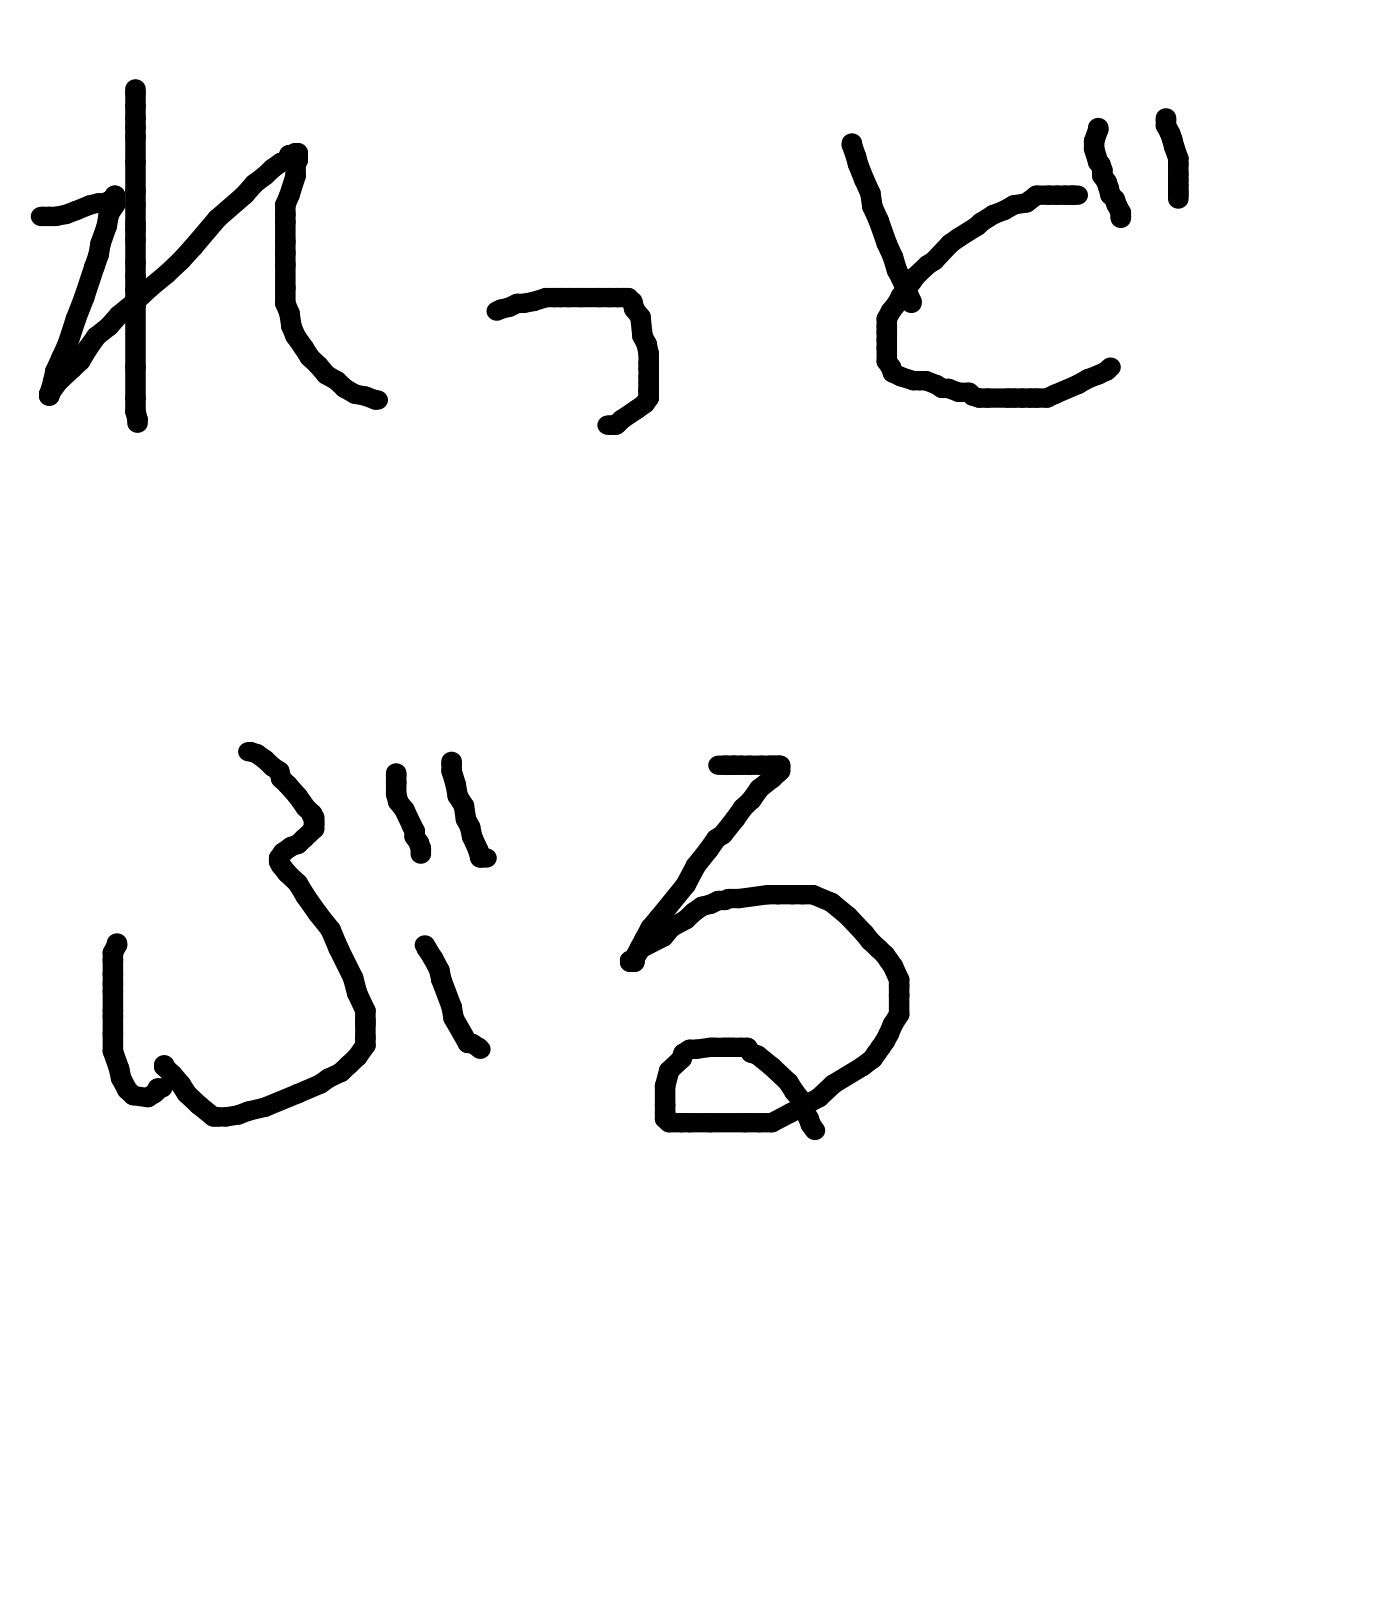
\includegraphics[width=5cm]{img/redbull.png}
		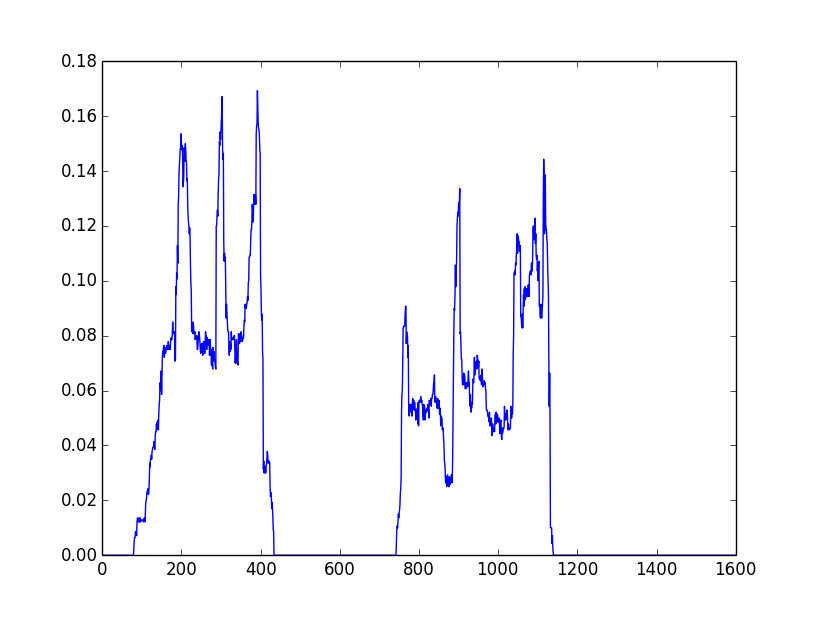
\includegraphics[width=8cm]{img/line.png}
		\caption{行抽出の様子}\label{fig1}
	\end{figure}
\end{center}

\begin{center}
	\begin{figure}[htbp]
		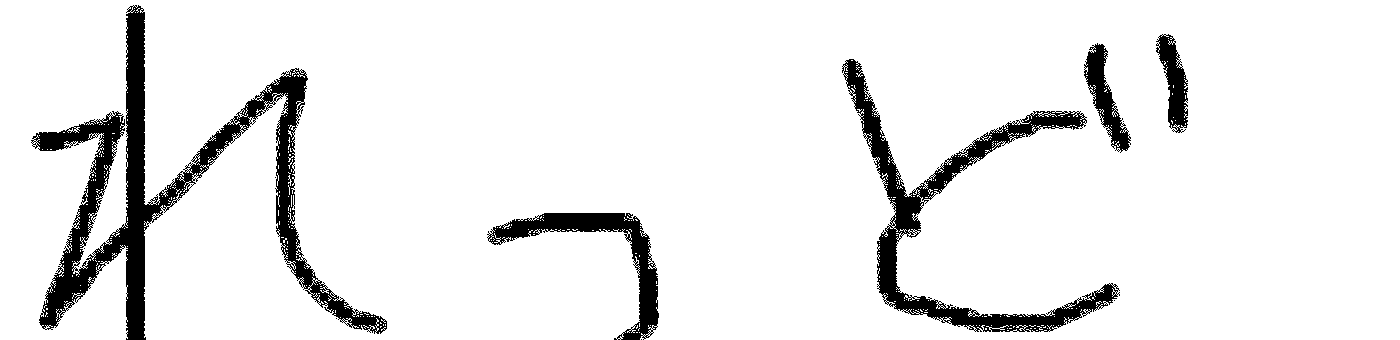
\includegraphics[width=5cm]{img/red.png}
		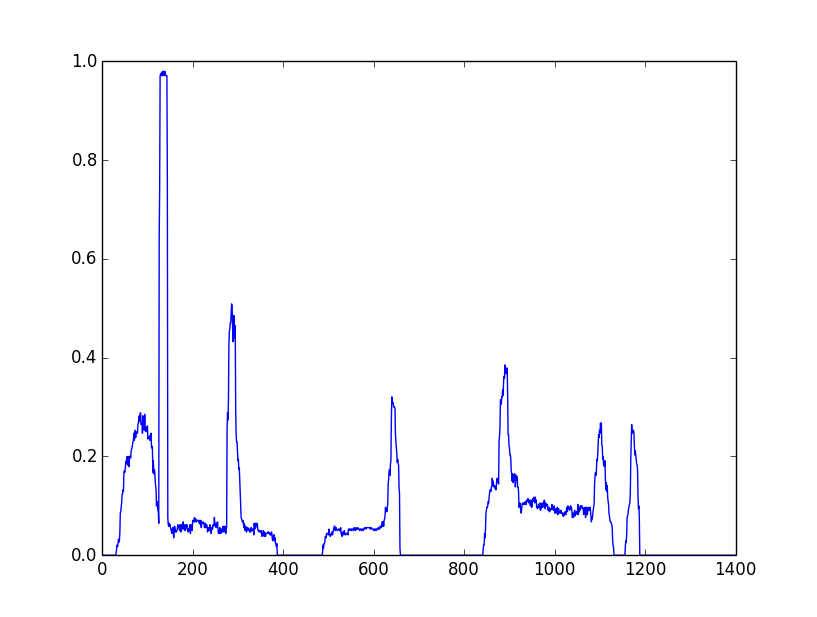
\includegraphics[width=8cm]{img/row.png}
		\caption{列抽出の様子}\label{fig2}
	\end{figure}
\end{center}

抽出処理ではスペクトルから山の範囲を決定して抽出を行っている.
「い」「は」「ふ」のように縦に見たときにスペクトルが2つの山になってしまう
文字については,まず2つの山にわけた抽出候補と1つの山にまとめた抽出候補を用意し,
両方で文字認識をさせた後に尤度の高い方を採用するようになっている.
「う」「え」のように横に見たときに2つの山に分かれてしまう文字についても同様である.

\subsection{文字認識}
当然のことながら文字認識は自動化しなければならないため,機械学習を用いて実装されている.
機械学習と聞くと漠然としたイメージを抱く方もいるかもしれないが,基本的なコンセプトとしては
既存の学習データを元にデータをうまく分類できる分類器をつくることである.
文字認識の場合は,既存の手書き文字データ群を学習させ,それらを正しく分類できるような
分類器をつくっておけば,未知の文字データを入力されたときに正しく分類できるという方向になる.
機械学習の詳細については,現在執筆中の拙著の記事
(https://github.com/levelfour/machine-learning-2014/wiki/第1回\#機械学習の基礎)
があるので参考になれば幸いである.

機械学習の学習アルゴリズムとして採用したのは,RandomForestである.
RandomForestを採用したことに理論的な背景は特別にあるわけではなく,
単に実験的に高い精度が得られたので採用している.


\section{問題点・改善点}
\subsection{認識精度}
現在の状態では決して認識精度が高いとは言い難い.
その原因は色々あるが,まずは文字抽出がそこまで正確ではないことが挙げられる.

現在は考えられうる抽出候補をすべて総当たり的に認識にかけることで
尤もらしい抽出結果を選択するようになっているが,
実際問題として認識対象文字列長が長くなるにつれて処理時間が
指数関数的に増大してしまう.
そういったことを考慮するとすべての抽出候補を検討するというのは現実的ではなく,
入力文字列画像のみから抽出できることが望ましい.
この記事(http://www.ohnishi.nuie.nagoya-u.ac.jp/~kudo/research/ifv/characters.segment.htm)では視覚の誘導場を利用した
文字抽出方法を提案しているので,参考にしてみると面白いかもしれない.

また,文字認識自体の精度に関しては,圧倒的に学習データ数が不足しているので
まずは学習データを「偏りなく」増やすことを考えたい.
そして,各段階におけるパラメータがあるので,そういったパラメータの
チューニングをしっかり行うべきである.
例えば,文字抽出時のしきい値やRandomForestのパラメータ等.
こういったパラメータを同時にチューニングするには計算資源を要するため,
未だ実現していない.

余談だが,学習データを増やす方法については,テストデータとして入力されたデータを
学習データとして再利用することを考えている.
つまり,何らかしらの手段でユーザが文字認識を行ったときに,
認識結果に対して正しいか間違っているかをたずね,可能であれば誤認していた場合に答えを教えさせるようにしたい.

\subsection{認識の前段階としての補正}
先程の話に繋がる部分が多分にあるが,文字認識を行う前に入力画像に対して補正をかける必要がある.
例えば,現在のアルゴリズムでは日本語の文字は基本的に正方形状であることを仮定しているが,
手書き文字では勿論人によって縦細かったり上下方向に歪んでいる等の文字の歪みがある.
文字に対して大まかな外接四角形をつくり,正方形状に変換することで
文字の歪みを補正することは認識精度の向上に役立つはずである.

\subsection{認識結果の精査}
認識結果についても結果をそのまま返すのではなく,吟味する必要がある.
例えば,「単言吾」という認識結果が返ってくれば,人間ならこれはどう見ても「単語」の誤認であるとわかる.
これと同じことを機械にも行わせると万が一誤認した場合でも修正をきかせることができる.
つまり,認識結果に対して辞書整合性を見るのである.
(勿論認識段階で誤認をなくせればそれがベストである)

\section{参考URL}
\begin{enumerate}
	\renewcommand{\labelenumi}{[\arabic{enumi}]}
	\item gihubリポジトリ https://github.com/levelfour/shrift
	\item 機械学習入門(拙著,執筆中) https://github.com/levelfour/machine-learning-2014/wiki
	\item ラボユースHackathonでの発表資料(SlideShare) http://www.slideshare.net/levelfour/shrift
	\item U-22プログラミング・コンテスト入選作品 http://www.u22procon.com/sakuhin.html
	\item ハンズラボ関連記事 https://www.hands-lab.com/contents/?p=893
\end{enumerate}

\end{document}
